%----------------------------------------------------------------------------------------
%	PACKAGES AND OTHER DOCUMENT CONFIGURATIONS
%----------------------------------------------------------------------------------------

\documentclass[final,hyperref={pdfpagelabels=false}]{beamer}

\usepackage[orientation=portrait,size=a0,scale=1.4]{beamerposter} % Use the beamerposter package for laying out the poster with a portrait orientation and an a0 paper size

% \toprule, \midrule, \bottomrule % instead of \hline
\usepackage{booktabs}
% Tables that can fit page length
\usepackage{tabularx}
% Multirows and multicolumns in table
\usepackage{multirow, multicol}

\usetheme{I6pd2} % Use the I6pd2 theme supplied with this template
\usepackage[english]{babel} % English language/hyphenation
\usepackage{amsmath,amsthm,amssymb,latexsym} % For including math equations, theorems, symbols, etc

%\usepackage{times}\usefonttheme{professionalfonts}  % Uncomment to use Times as the main font
%\usefonttheme[onlymath]{serif} % Uncomment to use a Serif font within math environments

%\boldmath % Use bold for everything within the math environment

\graphicspath{{media/}} % Location of the graphics files
\usecaptiontemplate{\small\structure{\insertcaptionname~\insertcaptionnumber:\,}\insertcaption} % A fix for figure numbering
\usepackage{siunitx}
\usepackage{caption}

%set reference on one line
\setbeamertemplate{bibliography entry article}{}
\setbeamertemplate{bibliography entry title}{}
\setbeamertemplate{bibliography entry location}{}
\setbeamertemplate{bibliography entry note}{}


% Acronyms
\usepackage{acronym}
\acrodef{SLAM}{simultaneous localization and mapping}
\acrodef{SOTA}{state-of-the-art}
\acrodef{TnR}{Teach-and-Repeat}
\acrodef{UGV}{Uncrewed ground vehicle} %FP: more gender neutral
\acrodef{UAVs}{Uncrewed aerial vehicles} %FP: more gender neutral
\acrodef{GNSS}{Global Navigation Satellite System}
\acrodef{IMU}{inertial measurement unit}
\acrodef{GP}{Gaussian processe}
\acrodef{ICP}{iterative closest point}

% models
% \bm % in equations for proper bold font
\usepackage{bm}

%----------------------------------------------------------------------------------------
%	TITLE SECTION 
%----------------------------------------------------------------------------------------

\title{\huge Field Report on a Wearable and Versatile Solution for Field Acquisition and Exploration} % Poster title

\author{\normalsize Olivier Gamache, Jean-Michel Fortin, Mat\v ej Boxan, François Pomerleau, Philippe Giguère} % Author(s)} % Author(s)

\institute{\small Northern Robotics Laboratory, Universit\'e Laval} % Institution(s)

%----------------------------------------------------------------------------------------
%	FOOTER TEXT
%----------------------------------------------------------------------------------------

\newcommand{\leftfoot}{IEEE International Conference on Robotics and Automation 2024} % Left footer text

\newcommand{\rightfoot}{olivier.gamache@norlab.ulaval.ca | philippe.giguere@ift.ulaval.ca} % Right footer text

%----------------------------------------------------------------------------------------

\begin{document}

\addtobeamertemplate{block end}{}{\vspace*{1ex}} % White space under blocks

\begin{frame}[t] % The whole poster is enclosed in one beamer frame

\begin{block}{Our Platform in Multiple Environments}
	\begin{figure}
	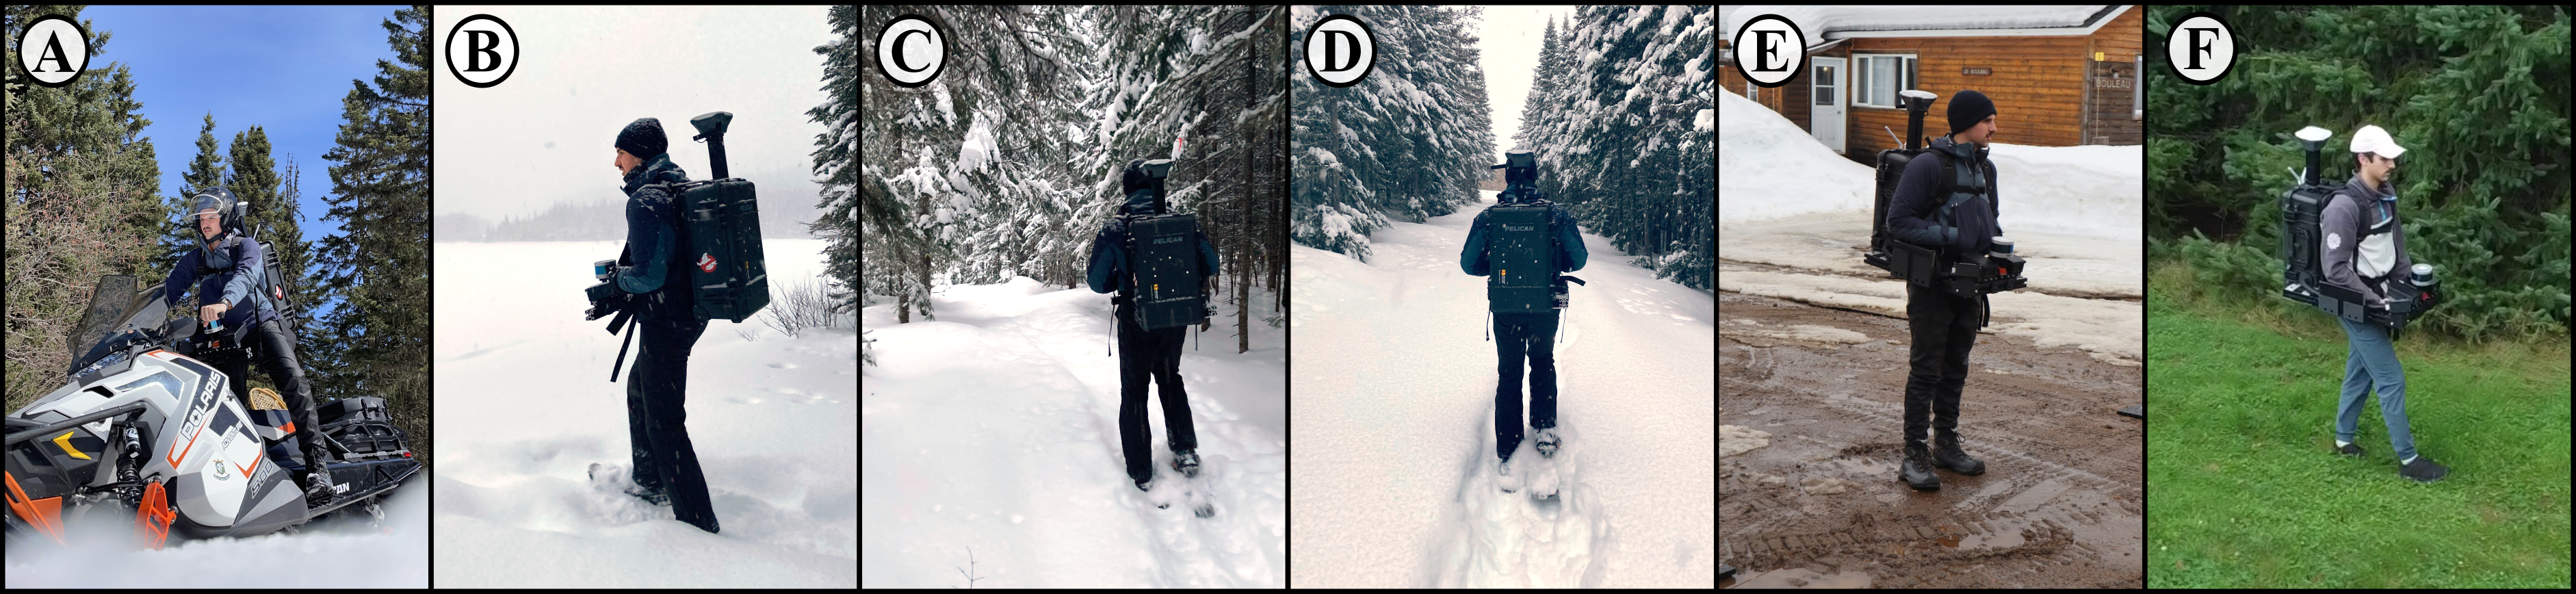
\includegraphics[width = 0.975\linewidth]{figures/backpack_images_mosaic.png}%
		%\vspace{-7mm}
		\captionsetup{width = 0.975\linewidth, justification=justified, name=Figure 1}
		\caption{
			Examples of environments traveled with the acquisition platform. \textbf{(A)} Winter displacement on a snowmobile, \textbf{(B)} Winter frozen lake, \textbf{(C)} winter dense forest, \textbf{(D)} Winter tree corridor, \textbf{(E)} Spring muddy forest, and \textbf{(F)} Summer forest.
		}
		\label{fig:mosaic}
	\end{figure}
\end{block}

\begin{columns}[t] % The whole poster consists of two major columns, each of which can be subdivided further with another \begin{columns} block - the [t] argument aligns each column's content to the top


\begin{column}{.0125\textwidth}\end{column} % Empty spacer column

\begin{column}{.465\textwidth} % The first column

%----------------------------------------------------------------------------------------
%	OBJECTIVES
%----------------------------------------------------------------------------------------
\vspace{-12.5mm}


\begin{block}{Context \& Motivations}
\begin{itemize}
	\item Real-life datasets are essential to improve autonomous navigation algorithms \cite{liu2024botanicgarden}.
	\item Capturing data in off-road environments require specialized \acp{UGV} \cite{Baril2022}, or \ac{UAVs}, which have highly limited battery life \cite{mozaffari2019tutorial}.
	\item Portable and easy-to-deploy system allows data recording on larger territory.
\end{itemize}
\end{block}

\begin{block}{Platform Description}
	\begin{itemize}
		\item We designed a plug-and-play multi-modalities platform averaging \SI{20}{\kilo\gram} with \SI{5.5}{\hour} of battery life.
		\item A control panel made of a LED screen and two push buttons provides sensors' status, and the hability to manage data acquisitions without needing external devices. 
		\item Cameras are triggered externally using hardware timers from a STM32F407 microcontroller, providing precise exposure time control and synchronization. 
	\end{itemize}
	\begin{figure}%
		\includegraphics[width=0.975\textwidth]{./figures/backpack_sensors_and_inside.pdf}
		\captionsetup{width = 0.975\linewidth, justification=justified, name=Figure 2}
		\caption{
			\textit{Left}: Picture of the developed backpack.
			Main components are identified as follows: \textbf{(1)} Two Basler a2A1920-51gcPRO cameras, \textbf{(2)} Xsens MTI-30 \ac{IMU}, \textbf{(3)} VLP16 3D lidar, \textbf{(4)} Emlid Reach RS+ GPS receiver, \textbf{(5)} Ubiquiti UniFi UAP-AC-M Wi-Fi antenna, \textbf{(6)} visualization tablet, and \textbf{(7)} control panel.
			\textit{Right}: Picture of the inside of the backpack. Main components are identified as follows: \textbf{(A)} TRENDnet TEG-S762 switch, \textbf{(B)} EGO battery \SI{2.5}{\ampere\hour}, \textbf{(C)} STM32F407 microcontroller, \textbf{(D)} Nvidia Jetson Xavier AGX Developer Kit, and \textbf{(E)} Asus XG-C100C \SI{10}{\giga b\per\second} PCIe.
			}
	\end{figure}
\end{block}

\begin{block}{Limitations}
	\begin{itemize}
		\item Absence of wheel odometry measurements.
		\item Maintaining a constant speed is demanding due to the platform's weight and the fatigue.
		\item Walking movements create oscillations in recorded data.
	\end{itemize}
\end{block}


%----------------------------------------------------------------------------------------

\end{column} % End of the first column

\begin{column}{.03\textwidth}\end{column} % Empty spacer column
 
\begin{column}{.465\textwidth} % The second column

%----------------------------------------------------------------------------------------
%	New block
%----------------------------------------------------------------------------------------

\vspace{-12.5mm}
\begin{block}{Lessons Learned}
	\begin{itemize}
		\item \textbf{Bandwidth} - To obtain robust communication, it is preferred to improve the hardware capibilities instead of overoptimizing on the software side.
		\item \textbf{Plug-and-play System} -  Investing time upfront in a user-friendly platform allows for faster data gathering later on, while a status display provides a more robust and efficient acquisition. 
		\item \textbf{Camera Power Supply} - Powering over Ethernet provides too much voltage, causing cameras to overheat and shutdown.
	\end{itemize}
\end{block}


\begin{block}{Applications}
	\begin{figure}%
		\begin{itemize}
			\item Efficient data recording allowed to collect BorealHDR \cite{gamache2023exposing}, a \SI{10}{\kilo\meter} off-road multi-seasonal and multi-modalities dataset.
		\end{itemize}
		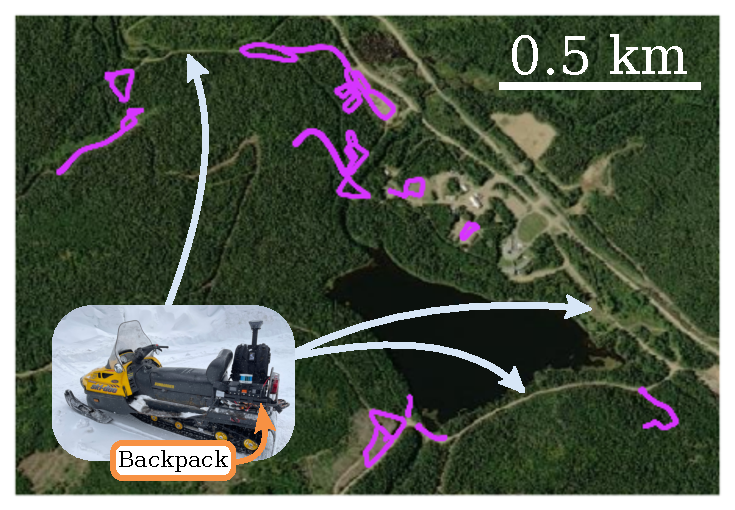
\includegraphics[width=0.6\textwidth]{./figures/figure_gps_trajectories.pdf}
		%\hfill
		\hskip1ex
		\begin{minipage}[b]{.35\textwidth}%
			\captionsetup{justification=justified, name=Figure 3}
			\caption{
				Satellite image of the Montmorency Forest, highlighting all the trajectories traveled on a one-day span in winter.
				The purple lines are the \ac{GNSS} positions from the \num{29} recorded trajectories, while the white arrows point to the roads traveled with the snowmobile.
				The backpack recording platform is attached to the end of the snowmobile only for the displacement between regions.
			}
		\end{minipage}%
	\end{figure}
	\begin{itemize}
		\item This portable platform was used in a \ac{TnR} setup to record the \textit{Teach} path. The \textit{Repeat} was then performed by an \ac{UGV}.
		% \item A similar application is useful for resupply mission, and is of interest for industry such as forestry, military and more!
	\end{itemize}
	\begin{figure}%
		\begin{minipage}[b]{.35\textwidth}%
			\captionsetup{justification=justified, name=Figure 4}
			\caption{
				Example of \ac{TnR} application.
				The \textit{teach phase} was recorded using our platform and is visible by following the imprint of walking steps in the snow.
				The \textit{repeat phase} was executed with a Clearpath Warthog platform.
				The purple box highlights the \textit{repeat path} centered on the walking steps from the \textit{teach path}.
				}
			\end{minipage}%
		\hskip1ex
		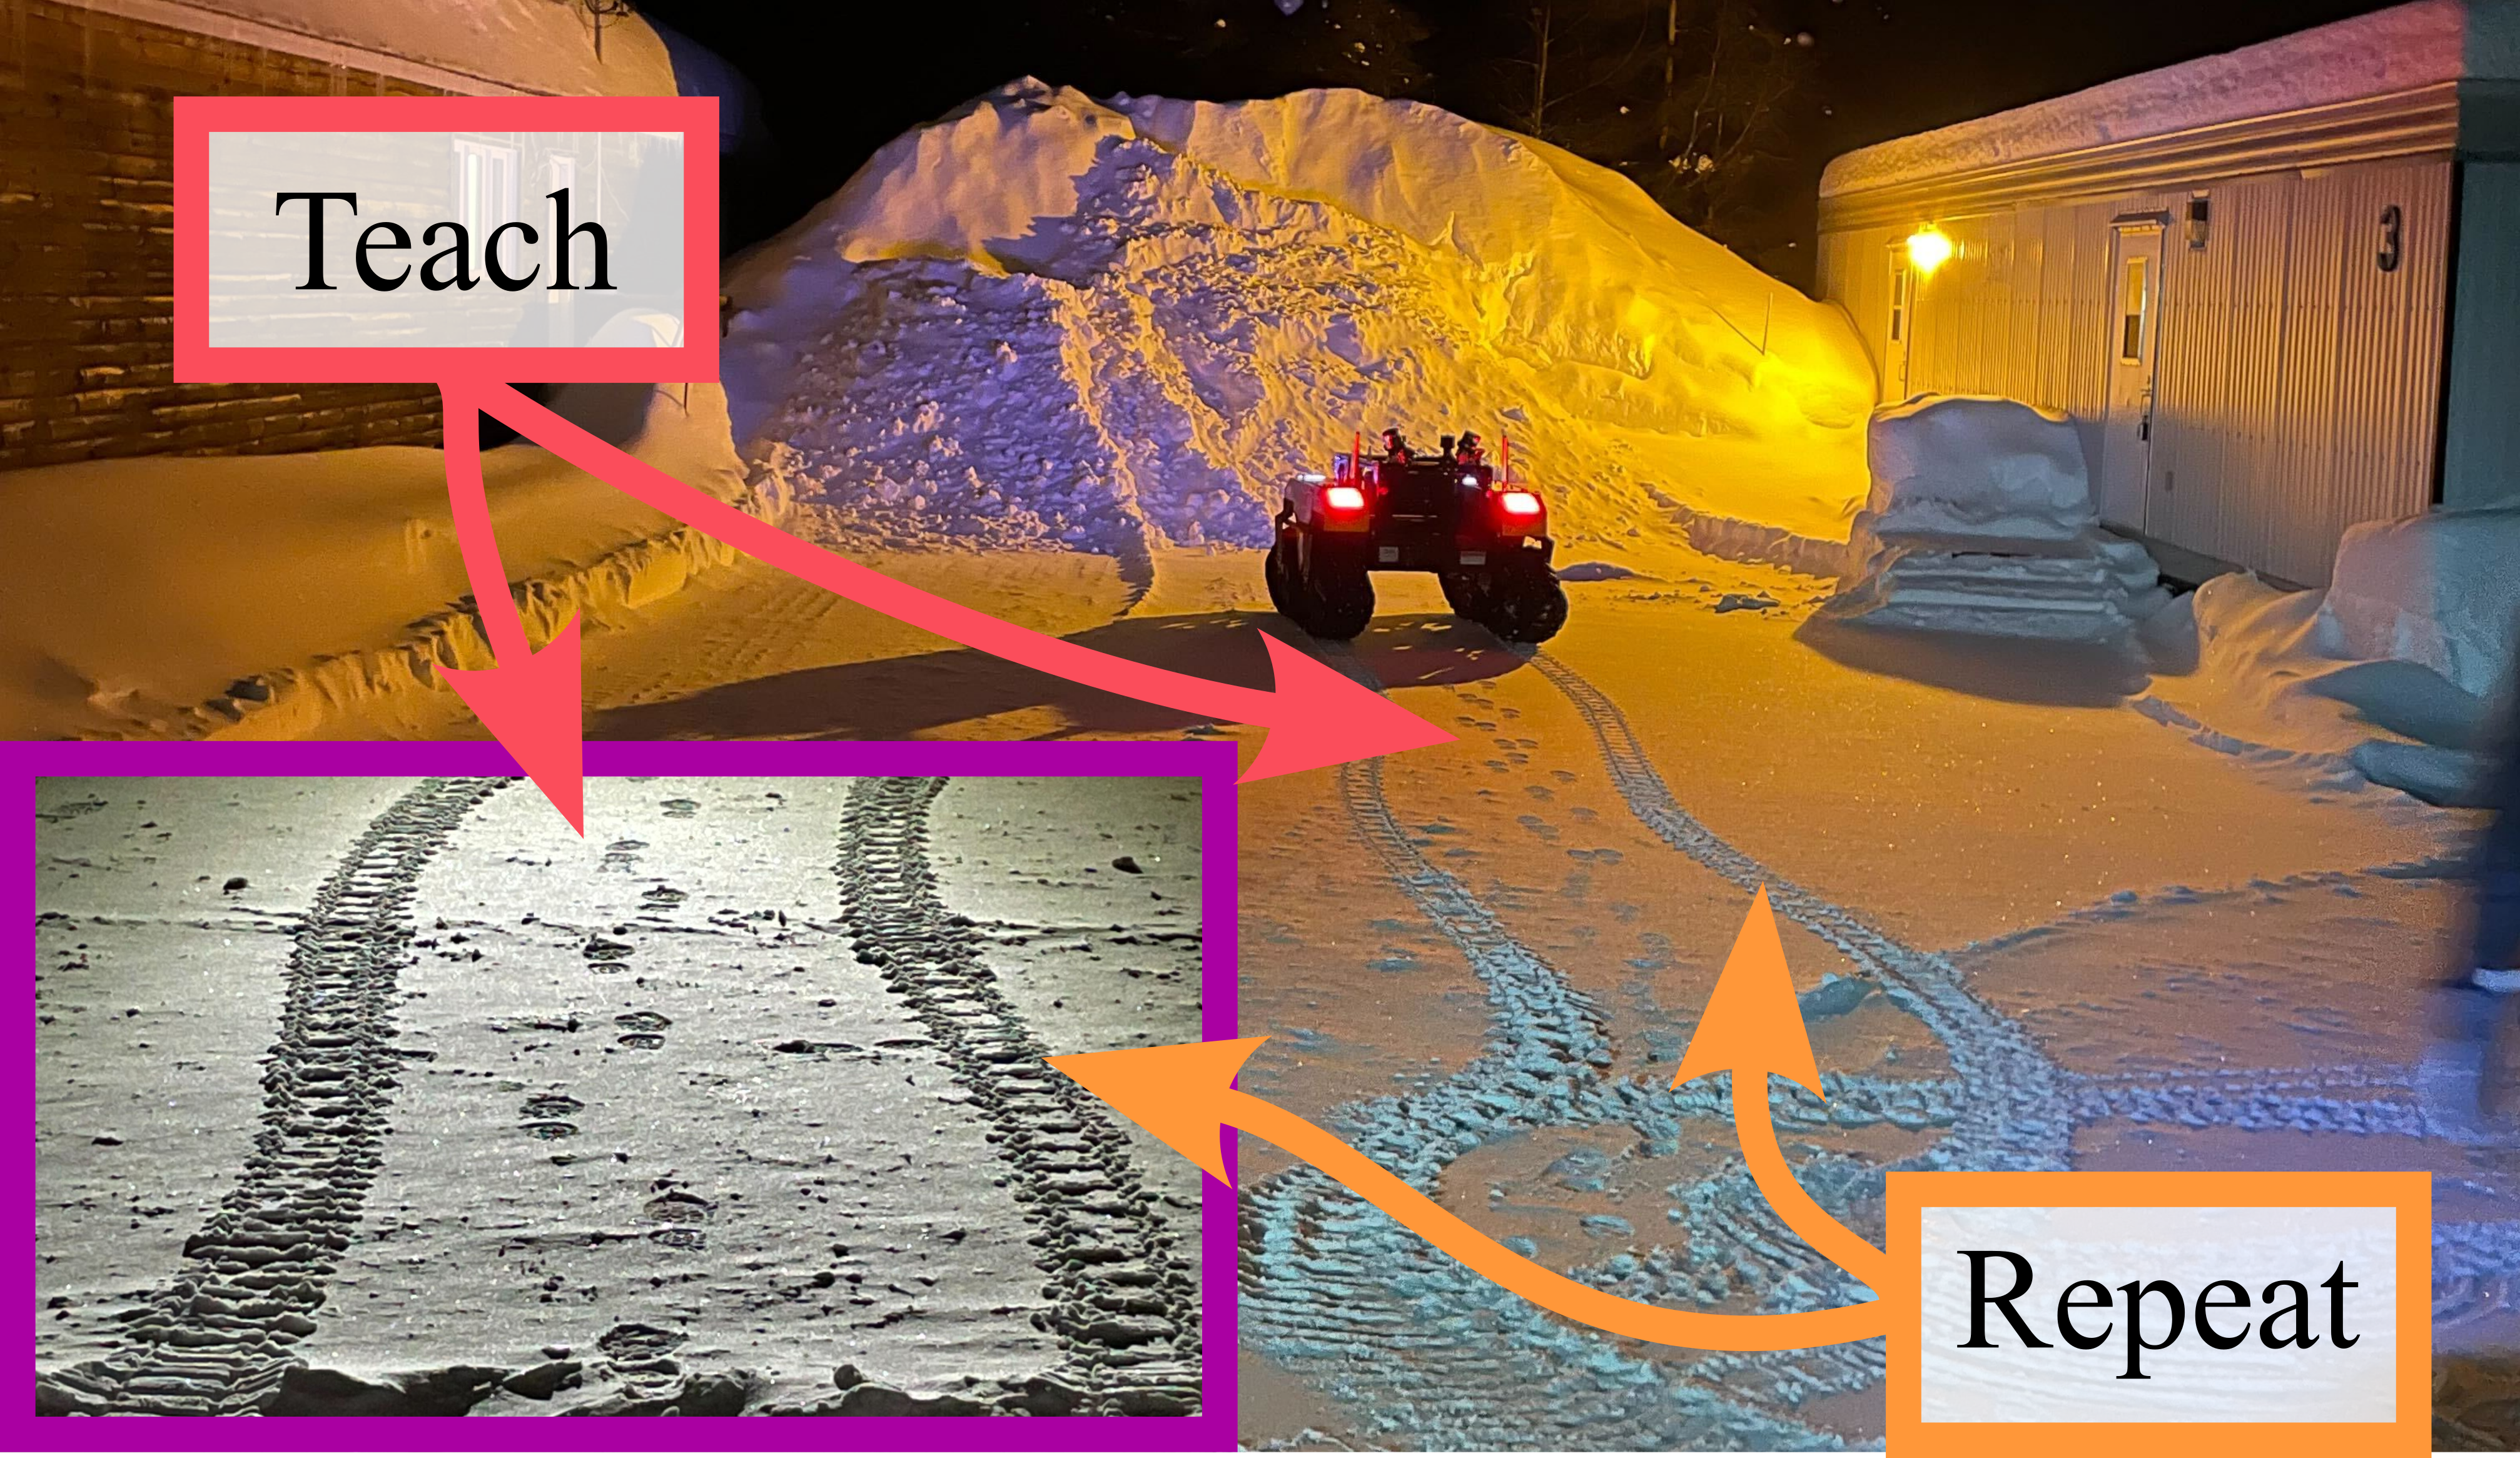
\includegraphics[width=0.6\textwidth]{./figures/fig_tnr.png}
	\end{figure}
	\begin{itemize}
		\item Such versatile and plug-and-play systems are of interest for industries, including forestry, military, and more!
	\end{itemize}
\end{block}

%----------------------------------------------------------------------------------------
%	ACKNOWLEDGEMENTS
%----------------------------------------------------------------------------------------


% \begin{block}{Acknowledgments and References}
% 	\footnotesize%
% 	\noindent This research was supported by Fonds de Recherche du Québec Nature et technologies (FRQNT) Team grant 254912 and Natural Sciences and Engineering Research Council of Canada (NSERC) DRC Grant through the grant CRD 538321-18, in collaboration with FP Innovations and Resolute Forest Products.
% 	%\vspace{-5mm}
% 	%\nocite{*} % Insert publications even if they are not cited in the poster
% 	\bibliographystyle{unsrt}%
% 	{\footnotesize\bibliography{biblio}}
% 	%\vspace{-3mm}
% \end{block}



%----------------------------------------------------------------------------------------
%	CONTACT INFORMATION
%----------------------------------------------------------------------------------------
%
%\setbeamercolor{block title}{fg=black,bg=orange!70} % Change the block title color
%
%\begin{block}{Contact Information}
%
%\begin{itemize}
%\item Web: \href{http://www.university.edu/smithlab}{http://www.university.edu/smithlab}
%\item Email: \href{mailto:john@smith.com}{john@smith.com}
%\item Phone: +1 (000) 111 1111
%\end{itemize}
%
%\end{block}

%----------------------------------------------------------------------------------------

\end{column} % End of the second column

\begin{column}{.015\textwidth}\end{column} % Empty spacer column
\end{columns} % End of all the columns in the poster
%----------------------------------------------------------------------------------------
%	REFERENCES
%----------------------------------------------------------------------------------------
%
%\begin{block}{References}
%\vspace{-5mm}
%\nocite{*} % Insert publications even if they are not cited in the poster
%\bibliographystyle{unsrt}%
%{\small\bibliography{biblio}}
%\vspace{-3mm}
%\end{block}

\begin{block}{Acknowledgments and References}
	\footnotesize%
	\noindent This research was supported by Fonds de Recherche du Québec Nature et technologies (FRQNT) Team grant 254912 and Natural Sciences and Engineering Research Council of Canada (NSERC) DRC Grant through the grant CRD 538321-18, in collaboration with FP Innovations and Resolute Forest Products.
	%\vspace{-5mm}
	%\nocite{*} % Insert publications even if they are not cited in the poster
	\bibliographystyle{unsrt}%
	{\footnotesize\bibliography{biblio}}
	%\vspace{-3mm}
\end{block}

\end{frame} % End of the enclosing frame

\end{document}
